Quelltexte können in zwei verschiedenen Kontexten in Fragestellungen auftauchen: Zum Einen gibt es unvollständige, kurze Quelltext-Fragmente, die in einen Fließtext eingebunden werden sollen, wie in diesem Beispiel:

\begin{quote}
„Wie viele String-Parameter hat die folgende Java-Methode?\newline
public String m(int i, int s, boolean b) \{ ... \}“
\end{quote}

Dabei handelt es sich um ein syntaktisch unvollständiges und nicht ausführbares Java-Fragment. Um die Lesbarkeit dieses Fragments zu erhöhen, sollte es dennoch optisch deutlich vom Fließtext unterscheidbar sein. Es bietet sich an, den Code in einer Monospace-Schriftart zu formatieren und (wenn möglich) eine syntaktische Einfärbung (Syntax Highlighting) anzuwenden.

Da die Entwicklung einer eigenen Editor-Komponente komplex ist, und es in diesem Bereich bereits eine große Auswahl an Bibliotheken gibt, wird auf eine bestehende Implementierung zurückgegriffen. Dabei müssen folgende Anforderungen von einer solchen Bibliothek erfüllt werden:

\begin{itemize}
    \item \textbf{Integration in React:}  Muss sich leicht in das deklarative React-Framework einbinden lassen.
    \item \textbf{WYSIWYG (What You See Is What You Get):} Der Editor muss stets eine Vorschau aller Formatierungen darstellen, und es soll nicht zwischen einem Markup- und einem Vorschau-Modus gewechselt werden müssen. Formatierungen sollen über Buttons eingefügt werden können.
    \item \textbf{Text-Formatierungen:} Der Editor muss über simple Text-Formatierungen verfügen (zum Beispiel Fettschrift und Kursivierung).
    \item \textbf{Monospace-Schriftart:} Eine Möglichkeit zum Verwenden einer Monospace-Schriftart muss vorhanden sein.
    \item \textbf{Syntax-Highlighting:} Syntaktische, farbliche Hervorhebungen von Code-Fragmenten müssen unterstützt werden (üblicherweise durch ein Plugin/Erweiterung mit einer zusätzlichen Bibliothek wie Highlight.js\footnote{Offizielle Webseite: \url{https://highlightjs.org/}}).
\end{itemize}

Nach dem Erwägen und Ausprobieren diverser Bibliotheken (z.B. Draft.js\footnote{Offizielle Webseite: \url{https://draftjs.org/}}, Slate\footnote{Offizielle Webseite: \url{https://www.slatejs.org/}}, Prosemirror\footnote{Offizielle Webseite: \url{https://prosemirror.net/}}) fiel die Wahl auf den Quill-Editor\footnote{Offizielle Webseite: \url{https://quilljs.com/}}, der alle genannten Anforderungen erfüllt. Quill ist nicht primär für den Einsatz mit React vorgesehen. Daher wird der Editor in Form der Wrapper-Bibliothek \texttt{react-quill}-Bibliothek\footnote{Offizielle Webseite: \url{https://github.com/zenoamaro/react-quill}} verwendet, die Quill in React-Komponenten bündelt.

\begin{figure}[H]
    \centering
    \setlength{\fboxsep}{0pt}
    \setlength{\fboxrule}{0.5pt}
    \fbox{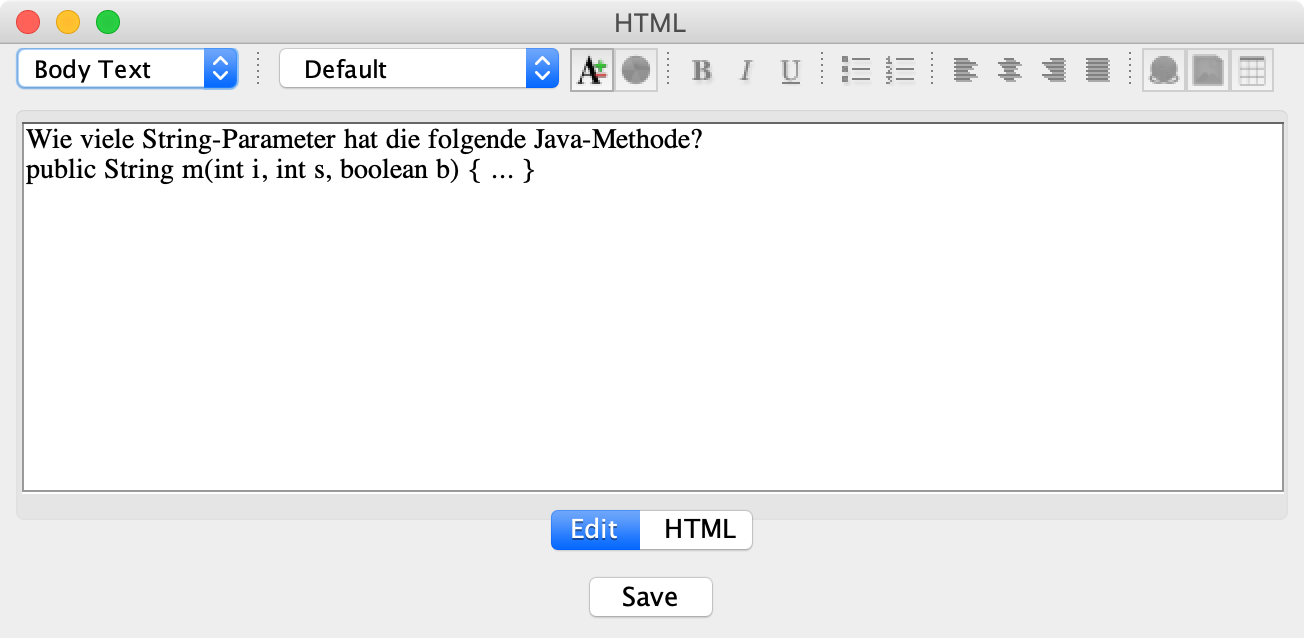
\includegraphics[width=\textwidth-1pt]{chapter/entwurf/bilder/sturesy_editor.png}}
    \caption[StuReSy-Fragen-Editor]{Bearbeitung einer Fragestellung im StuReSy-Fragen-Editor.}
    \label{abb:sturesy_editor}
\end{figure}

\begin{figure}[H]
    \centering
    \setlength{\fboxsep}{0pt}
    \setlength{\fboxrule}{0.5pt}
    \fbox{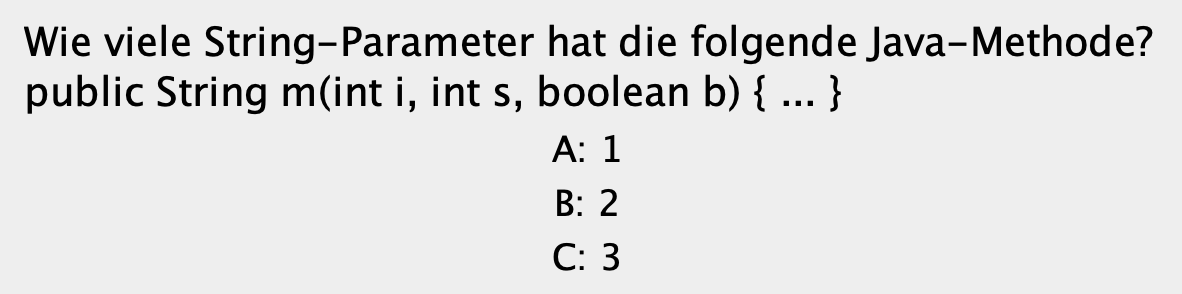
\includegraphics[width=\textwidth-1pt]{chapter/entwurf/bilder/sturesy_fragment.png}}
    \caption[Darstellung eines Code-Fragments in StuReSy]{Darstellung eines Code-Fragments in StuReSy (ohne manuell vorgenommene Formatierungen).}
    \label{abb:sturesy_code_fragment}
\end{figure}


\begin{figure}[H]
    \centering
    \setlength{\fboxsep}{0pt}
    \setlength{\fboxrule}{0.5pt}
    \fbox{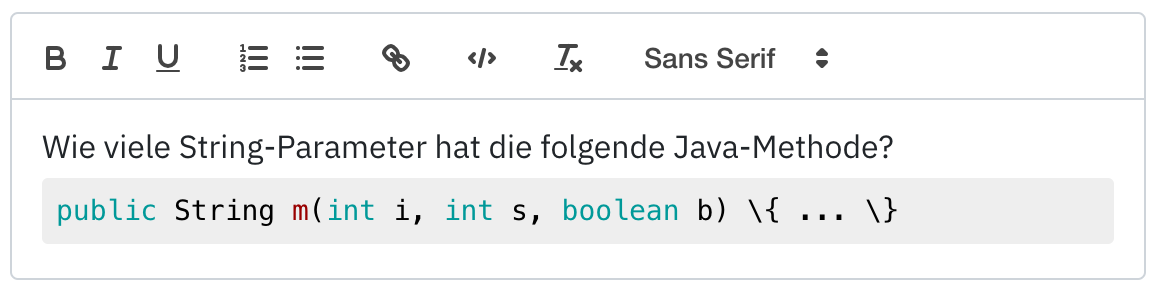
\includegraphics[width=\textwidth-1pt]{chapter/entwurf/bilder/weclare_quill.png}}
    \caption[Quill-Editor von Weclare]{Bearbeitung einer Fragestellung im Quill-Editor von Weclare.}
    \label{abb:weclare_quill}
\end{figure}

\begin{figure}[H]
    \centering
    \setlength{\fboxsep}{0pt}
    \setlength{\fboxrule}{0.5pt}
    \fbox{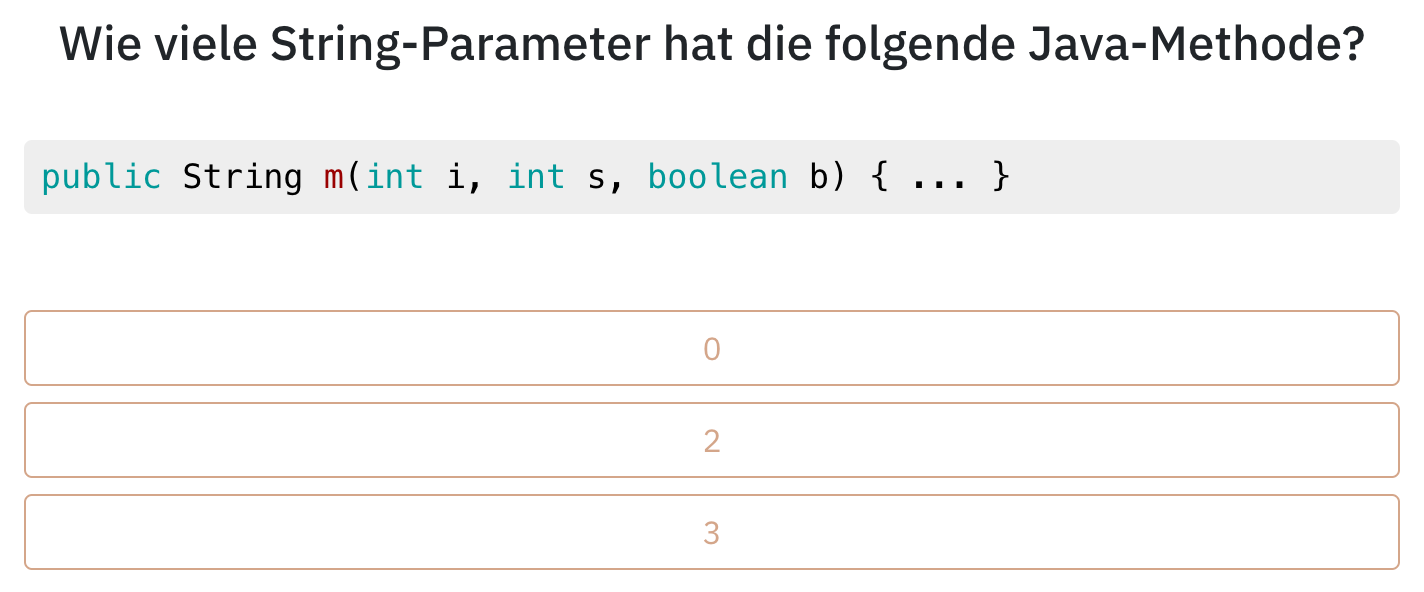
\includegraphics[width=\textwidth-1pt]{chapter/entwurf/bilder/weclare_fragment.png}}%
    \caption[Darstellung eines Code-Fragments in Weclare]{Darstellung eines Code-Fragments in Weclare (Quelltext als Code-Block ausgezeichnet).}
    \label{abb:weclare_code_fragment}
\end{figure}

Der zweite Kontext von Quelltexten in Fragestellungen ist das Einfügen von vollständigem, ausführbarem Code, in Form ganzer Java-Klassen. Derartiger Code kann in Weclare direkt im Browser ausgeführt werden. Solch ein interaktives Code-Beispiel kann allerdings nur einmal pro Frage vorhanden sein und ist auch nicht Teil des Fließtexts. Eine entsprechende Editor-Komponente zum Einfügen des Codes sollte also auch funktional darauf zugeschnitten sein: Text-Formatierungen sind nicht mehr notwendig, stattdessen rücken Funktionen wie die korrekte Einrückung von Code-Zeilen und Zeilen-Nummerierungen in den Vordergrund.

Der Quill-Editor kann nicht in einem „Code only“-Modus betrieben werden, so dass eine zweite, unabhängige Editor-Komponente für interaktive Code-Abschnitte integriert wird. Mit CodeMirror\footnote{Offizielle Webseite: \url{https://codemirror.net/}} existiert eine beliebte Bibliothek für diesen Zweck, die allerdings nicht explizit für den Einsatz im React-Framework bestimmt ist, so dass auch sie in Form einer Wrapper-Bibliothek namens \texttt{react-codemirror2}\footnote{Offizielle Webseite: \url{https://github.com/scniro/react-codemirror2}} zum Einsatz kommt.



\begin{figure}[H]
    \centering
    \setlength{\fboxsep}{0pt}
    \setlength{\fboxrule}{0.5pt}
    \fbox{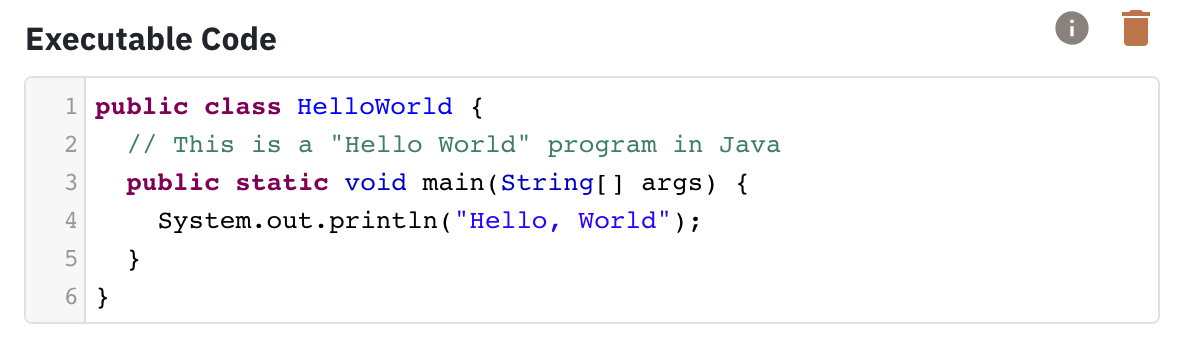
\includegraphics[width=\textwidth-1pt]{chapter/entwurf/bilder/weclare_codemirror.png}}
    \caption[Darstellung eines ausführbaren Java-Quelltexts in Weclare]{Darstellung eines ausführbaren Java-Quelltexts in Weclare mittels der CodeMirror-Bibliothek.}
    \label{abb:weclare_codemirror}
\end{figure}